\section{函数项级数}
\subsection{函数项级数的概念}
\begin{definition}\label{definition:无穷级数.实函数项级数的概念}
%@see: 《数学分析(第二版 下册)》(陈纪修) P55 定义10.1.1
%@see: 《数学分析(第7版 第二卷)》(卓里奇) P299 定义1
%@see: 《数学分析(第7版 第二卷)》(卓里奇) P299 定义2
%@see: 《数学分析(第7版 第二卷)》(卓里奇) P299 定义4
给定一个定义在区间\(I \subseteq \mathbb{R}\)上的函数列\[
	u_1,u_2,\dotsc,u_n,\dotsc,
\]
则由该函数列构成的表达式\[
	u_1(x)+u_2(x)+\dotsb+u_n(x)+\dotsb
\]
称为“定义在区间\(I\)上的\DefineConcept{函数项无穷级数}
(infinite series with function terms)”,
简称\DefineConcept{函数项级数},
或者进一步简称为\DefineConcept{级数},
记作\[
	x \mapsto \sum_{n=1}^\infty u_n(x),
\]
或\[
	\sum_{n=1}^\infty u_n.
\]
\end{definition}
\begin{remark}
函数项无穷级数本质上是一个映射.
它的定义域是各项函数\(u_k\)的共同定义域\[
	I \subseteq \bigcap\Set{ \dom u_k \given k=1,2,\dotsc }.
\]
于是,对于每一个确定的值\(x_0 \in I\),
只要在函数项无穷级数的表达式\(\sum_{n=1}^\infty u_n(x)\)中,用\(x_0\)代入\(x\),
就能得到一个常数项无穷级数\(\sum_{n=1}^\infty u_n(x_0)\).
只不过,并非所有\(x_0\)都能保证
常数项无穷级数\(\sum_{n=1}^\infty u_n(x_0)\)是收敛的.
\end{remark}

\begin{definition}
如果常数项无穷级数\(\sum_{n=1}^\infty u_n(x_0)\)收敛,
则称“函数项级数\(\sum_{n=1}^\infty u_n\)在点\(x_0\)收敛”
或“点\(x_0\)是函数项级数\(\sum_{n=1}^\infty u_n\)的\DefineConcept{收敛点}
(point of convergence)”.

如果常数项无穷级数\(\sum_{n=1}^\infty u_n(x_0)\)发散,
就称“函数项级数\(\sum_{n=1}^\infty u_n\)在点\(x_0\)发散”
或“点\(x_0\)是函数项级数\(\sum_{n=1}^\infty u_n\)的\DefineConcept{发散点}
(point of divergence)”.

函数项级数\(\sum_{n=1}^\infty u_n\)的收敛点的全体称为
“函数项级数\(\sum_{n=1}^\infty u_n\)的\DefineConcept{收敛域}(domain of convergence)”,
记作\(\dom \sum_{n=1}^\infty u_n\).

函数项级数\(\sum_{n=1}^\infty u_n\)的发散点的全体称为
“函数项级数\(\sum_{n=1}^\infty u_n\)的\DefineConcept{发散域}(domain of divergence)”.
\end{definition}

\begin{definition}
记\(D \defeq \dom\sum_{n=1}^\infty u_n\).
把函数\[
	S\colon D\to\mathbb{R},
	x \mapsto \sum_{n=1}^\infty u_n(x),
\]称为“函数项级数\(\sum_{n=1}^\infty u_n\)的\DefineConcept{和函数}”.

由于这个函数是通过逐点定义的方式得到的,
因此我们称“函数项级数\(\sum_{n=1}^\infty u_n\)在\(D\)上
具有\DefineConcept{点态收敛性}(pointwise convergence)”,
“函数项级数\(\sum_{n=1}^\infty u_n\)在\(D\)上\DefineConcept{点态收敛}于\(S\)”.

把函数\[
	S_n\colon I\to\mathbb{R},
	x \mapsto \sum_{k=1}^n u_k(x)
\]称为“函数项级数\(\sum_{n=1}^\infty u_n\)的\DefineConcept{部分和函数}(partial sum)”.
\end{definition}

\begin{definition}
当函数项级数\(\sum_{n=1}^\infty u_n\)收敛时,
把函数\[
	R_n\colon D\to\mathbb{R},
	x \mapsto S(x) - S_n(x),
\]称为“函数项级数\(\sum_{n=1}^\infty u_n\)的\DefineConcept{余项函数}”.
\end{definition}

\begin{definition}
%@see: 《数学分析(第7版 第二卷)》(卓里奇) P299 定义3
设函数列\(\{S_n\}\)在集合\(D\)上点态收敛于函数\(S\),
即对任意\(x \in D\)成立\[
	\lim_{n\to\infty} S_n(x) = S(x),
\]
则把\(S\)称为“函数列\(\{S_n\}\)的\DefineConcept{极限函数}”,
记作\[
	S_n \to S\ (n\to\infty,x \in D)
	\quad\text{或}\quad
	S_n \overset{D}\to S,
\]
不强调区间\(D\)时,也可以记作\(S_n \to S\).
\end{definition}

\begin{proposition}
%@see: 《数学分析(第二版 下册)》(陈纪修) P56
设\(\{S_n\}\)是函数项级数\(\sum_{n=1}^\infty u_n\)的部分和函数列,
则\[
	\Set{ x \given \text{数列$\{S_n(x)\}$收敛} } = D.
\]
\end{proposition}
\begin{proposition}
%@see: 《数学分析(第二版 下册)》(陈纪修) P56
设\(S\)是函数项级数\(\sum_{n=1}^\infty u_n\)的和函数,
\(S_n\)是函数项级数\(\sum_{n=1}^\infty u_n\)的部分和函数,
则在收敛域\(D\)上有\[
	\lim_{n\to\infty} S_n(x) = S(x).
\]
\end{proposition}
\begin{proposition}
设\(R_n\)是函数项级数\(\sum_{n=1}^\infty u_n\)的余项函数,
则在收敛域\(D\)上有\[
	\lim_{n\to\infty} R_n(x) = 0.
\]
\end{proposition}
\begin{remark}
可以看出,函数项级数\(\sum_{n=1}^\infty u_n\)与函数列\(\{S_n\}\)的收敛性在本质上完全是一回事.
\end{remark}

\begin{example}
%@see: 《数学分析(第二版 下册)》(陈纪修) P55 例10.1.1
利用常数项无穷级数审敛法和\cref{definition:无穷级数.实函数项级数的概念},可知下述结论:
\begin{itemize}
	\item \(\sum_{n=1}^\infty x^n\)的收敛域为\((-1,1)\),
	和函数为\(S(x) = \frac{x}{1-x}\).
	\item \(\sum_{n=1}^\infty \frac{x^n}{n}\)的收敛域为\([-1,1)\).
	\item \(\sum_{n=1}^\infty \frac{x^n}{n^2}\)的收敛域为\([-1,1]\).
	\item \(\sum_{n=1}^\infty \frac{x^n}{n!}\)的收敛域是\((-\infty,+\infty)\).
	\item \(\sum_{n=1}^\infty n! x^n\)的收敛域是\(\{0\}\).
	\item \(\sum_{n=1}^\infty e^{-nx}\)的收敛域为\((0,+\infty)\),
	和函数为\(S(x) = \frac1{e^x-1}\).
\end{itemize}
\end{example}

\begin{example}
%@see: 《数学分析教程(第3版 上册)》(史济怀) P213 问题15.1 1.
设函数项级数\(\sum_{n=1}^\infty u_n(x)\)在有界闭区间\([a,b]\)上收敛于\(S(x)\),
且\(u_n\ (n=1,2,\dotsc)\)都是\([a,b]\)上的非负连续函数.
证明:\(S\)必在\([a,b]\)上有最小值.
\begin{proof}
记\(S_n(x) = \sum_{k=1}^n u_k(x)\),
则有\[
	0 \leq S_n(x) \leq S_{n+1}(x) \leq S(x),
\]
所以\(S\)在\([a,b]\)上有下确界\(\alpha\).
于是对于每个正整数\(n\),
存在\(x_n\in[a,b]\),
使得\[
	\alpha \leq S(x_n) < \alpha + \frac1n,
\]
即\[
	\lim_{n\to\infty} S(x_n) = \alpha.
\]
因为\(x_n\in[a,b]\),
所以存在子列\(\{x_{n_k}\}\)使得\[
	\lim_{k\to\infty} x_{n_k} = x_0 \in [a,b].
\]
我们要证明\(S(x_0) = \alpha\).
对任意的正整数\(m\),
有\[
	S_m(x_{n_k})
	\leq S(x_{n_k})
	< \alpha + \frac1{n_k}.
\]
令\(n\to\infty\),
由于\(S_m\)在点\(x_0\)连续,
所以\[
	S_m(x_0) \leq \alpha.
\]
再令\(m\to\infty\),
便得\[
	S(x_0) \leq \alpha.
\]
但是\(S(x_0) \geq \alpha\),
所以\(S(x_0) = \alpha\).
\end{proof}
\end{example}

\subsection{函数项级数和函数列的基本问题}
%@see: 《数学分析(第二版 下册)》(陈纪修) P56
通过前面的学习我们已经知道,
若有限个函数\(u_1,u_2,\dotsc,u_n\)在\(D\)上有定义且具有某种分析性质,
如连续性、可导性和黎曼可积性,
则它们的和函数\[
	u_1(x) + u_2(x) + \dotsb + u_n(x)
\]在\(D\)上仍保持同样的分析性质,
且其和函数的极限、导数或黎曼积分
可以通过对每个函数分别求极限、导数或黎曼积分后再求和来得到,
即\begin{gather*}
	\lim_{x \to x_0} [u_1(x) + u_2(x) + \dotsb + u_n(x)]
	= \lim_{x \to x_0} u_1(x)
	+ \lim_{x \to x_0} u_2(x)
	+ \dotsb
	+ \lim_{x \to x_0} u_n(x), \\
	\dv{x} [u_1(x) + u_2(x) + \dotsb + u_n(x)]
	= \dv{x} u_1(x)
	+ \dv{x} u_2(x)
	+ \dotsb
	+ \dv{x} u_n(x), \\
	\int_a^b [u_1(x) + u_2(x) + \dotsb + u_n(x)] \dd{x}
	= \int_a^b u_1(x) \dd{x}
	+ \int_a^b u_2(x) \dd{x}
	+ \dotsb
	+ \int_a^b u_n(x) \dd{x}.
\end{gather*}

在研究函数项级数时,我们面对的是无限个函数之和.
它们的和函数\(S\)大多是未知的,也就是说,
我们只能借助函数\(u_n\)的分析性质来间接地获得\(S\)的分析性质.
那么我们自然希望上述运算法则可以在一定条件下推广到无限个函数求和的情况.

这个问题是函数项级数和函数列研究中的基本问题,
其实质是极限、求导、求积分运算与无限求和运算在什么条件下可以交换次序.
由于求导、求积分与无限求和均可看作特殊的极限运算,因此更一般地,
可以将其统一视为两种极限运算的交换次序.
下面我们将会看到,仅要求\(\sum_{n=1}^\infty u_n(x)\)在\(D\)上点态收敛是不够的.

\begin{definition}
%@see: 《数学分析(第二版 下册)》(陈纪修) P57
设\(S\)是函数项级数\(\sum_{n=1}^\infty u_n\)的和函数.
如果当\(u_n\)在\(D\)上连续时,函数\(S\)也在\(D\)上连续,
并且成立\[
	\lim_{x \to x_0} \sum_{n=1}^\infty u_n(x)
	= \sum_{n=1}^\infty \lim_{x \to x_0} u_n(x),
\]
则称“极限运算与无限求和运算可以交换次序”
或“函数项级数\(\sum_{n=1}^\infty u_n\)可以\DefineConcept{逐项求极限}”.
\end{definition}
对于函数列\(\{S_n\}\)而言,相应的结论是
极限函数\(S(x) = \lim_{n\to\infty} S_n(x)\)也在\(D\)上连续,
并且成立\[
	\lim_{x \to x_0} \lim_{n\to\infty} S_n(x)
	= \lim_{n\to\infty} \lim_{x \to x_0} S_n(x),
\]
即两种极限运算可以交换次序.

下面的例子说明,在点态收敛的情况下,函数项级数不一定可以逐项求极限.
\begin{example}\label{example:函数项级数.点态收敛情况下和函数可能不连续}
%@see: 《数学分析(第二版 下册)》(陈纪修) P58 例10.1.2
%@see: 《数学分析(第7版 第二卷)》(卓里奇) P299 例1
设\(S_n(x) = x^n\),
则函数列\(\{S_n\}\)在区间\((-1,1]\)上收敛,
极限函数为\[
	S(x) = \lim_{n\to\infty} S_n(x)
	= \left\{ \begin{array}{ll}
		0, & -1<x<1, \\
		1, & x=1.
	\end{array} \right.
\]
虽然对于任意正整数\(n\),函数\(S_n\)在\((-1,1]\)上连续(也是可导的),
但极限函数\(S\)在\(x=1\)不连续(当然更谈不上在\(x=1\)可导).
\end{example}

\begin{definition}
%@see: 《数学分析(第二版 下册)》(陈纪修) P58
设\(S\)是函数项级数\(\sum_{n=1}^\infty u_n\)的和函数.
如果当\(u_n\)在\(D\)上可导时,函数\(S\)也在\(D\)上可导,
并且成立\[
	\dv{x} \sum_{n=1}^\infty u_n(x)
	= \sum_{n=1}^\infty \dv{x} u_n(x),
\]
则称“求导运算与无限求和运算可以交换次序”
或“函数项级数\(\sum_{n=1}^\infty u_n\)可以\DefineConcept{逐项求导}”.
\end{definition}
对于函数列\(\{S_n\}\)而言,相应的结论是
极限函数\(S(x) = \lim_{n\to\infty} S_n(x)\)也在\(D\)上可导,
并且成立\[
	\dv{x} \lim_{n\to\infty} S_n(x)
	= \lim_{n\to\infty} \dv{x} S_n(x),
\]
即求导运算与极限运算可以交换次序.

\cref{example:函数项级数.点态收敛情况下和函数可能不连续} 已说明:
在点态收敛情况下,和函数(或极限函数)可能不可导.
下面将看到,即使和函数(或极限函数)可导,上述两个等式也不一定成立.
\begin{example}
%@see: 《数学分析(第二版 下册)》(陈纪修) P58 例10.1.3
设\(S_n(x) = \frac{\sin nx}{\sqrt{n}}\),
则函数列\(\{S_n\}\)在区间\((-\infty,+\infty)\)上收敛,
极限函数为\(S(x) = 0\),从而导函数\(S'(x) = 0\).
由于\[
	S_n'(x) = \sqrt{n} \cos nx,
\]
因此\(S_n\)的导函数所构成的序列\(\{S_n'\}\)并不收敛于\(S'\),
例如当\(x=0\)时\[
	S_n'(0) = \sqrt{n}\to+\infty\ (n\to\infty).
\]
\end{example}

\begin{definition}
%@see: 《数学分析(第二版 下册)》(陈纪修) P58
设\(S\)是函数项级数\(\sum_{n=1}^\infty u_n\)的和函数.
如果当\(u_n\)在闭区间\([a,b] \subseteq D\)上黎曼可积时,函数\(S\)也在\([a,b]\)上黎曼可积,
并且成立\[
	\int_a^b \sum_{n=1}^\infty u_n(x) \dd{x}
	= \sum_{n=1}^\infty \int_a^b u_n(x) \dd{x},
\]
则称“求积分运算与无限求和运算可以交换次序”
或“函数项级数\(\sum_{n=1}^\infty u_n\)可以\DefineConcept{逐项求积分}”.
\end{definition}
对于函数列\(\{S_n\}\)而言,相应的结论是
极限函数\(S(x) = \lim_{n\to\infty} S_n(x)\)也在闭区间\([a,b]\)上黎曼可积,
并且成立\[
	\int_a^b \lim_{n\to\infty} S_n(x) \dd{x}
	= \lim_{n\to\infty} \int_a^b S_n(x) \dd{x},
\]
即求积分运算与极限运算可以交换次序.

下面将看到,在点态收敛情况下,
和函数(或极限函数)可能不可积;
即使黎曼可积,上述两个等式也不一定成立.
\begin{example}
%@see: 《数学分析(第二版 下册)》(陈纪修) P59 例10.1.4
设函数\(S_n\colon[0,1]\to\{0,1\}\)满足\[
	S_n(x) = \left\{ \begin{array}{cl}
		1, & \text{$n! \cdot x$是整数},  \\
		0, & \text{其他}.
	\end{array} \right.
\]
显然,对于每一个正整数\(n\),函数\(S_n\)在\([0,1]\)上有界,
至多只有有限个不连续点,因而是可积的.

但是,当\(x\)是无理数时,对一切正整数\(n\),有\(S_n(x) = 0\),
因此\(S(x) = \lim_{n\to\infty} S_n(x) = 0\);
当\(x\)是有理数时,不妨设\(x\)等于既约分数\(q/p\),
即\(p\in\mathbb{N}^+,
q\in\mathbb{N},
q \leq p\),
那么对于\(n \geq p\),有\(S_n(x) = 1\),
因此\(S(x) = \lim_{n\to\infty} S_n(x) = 1\).
所以\(\{S_n\}\)的极限函数\(S\)就是我们熟知的狄利克雷函数,
它在\([0,1]\)上是不可积的.
\end{example}
\begin{example}
%@see: 《数学分析(第二版 下册)》(陈纪修) P59 例10.1.5
设\(S_n(x) = nx(1-x^2)^n\),
则\(\{S_n\}\)在区间\([0,1]\)上收敛于极限函数\(S(x) = 0\).
但是\begin{align*}
	\int_0^1 S_n(x) \dd{x}
	&= \int_0^1 n x (1-x^2)^n \dd{x}
	= -\frac{n}{2} \int_0^1 (1-x^2)^n \dd(1-x^2) \\
	&= \frac{n}{2(n+1)}
	\not\to \int_0^1 S(x) \dd{x}
	\quad(n\to\infty).
\end{align*}
\end{example}
这些例子说明,为了解决这类交换运算次序问题,
需要引进比“点态收敛”要求更强的新的收敛概念.

\subsection{函数项级数或函数列的一致收敛性}
%@see: 《数学分析(第二版 下册)》(陈纪修) P59
\begin{definition}\label{definition:无穷级数.函数项级数的一致收敛性}
%@see: 《数学分析(第二版 下册)》(陈纪修) P60 定义10.1.2
%@see: 《高等数学(第六版 上册)》 P294 定义
设定义在区间\(D\)上的函数列\(\{S_n\}\).
若对任意给定\(\epsilon>0\),
存在仅与\(\epsilon\)有关的的正整数\(N\),
当\(n>N\)时,
对\(D\)上的一切\(x\),
成立\[
	\abs{S(x) - S_n(x)} < \epsilon,
\]
则称“函数列\(\{S_n\}\)在\(D\)上
具有\DefineConcept{一致收敛性}(uniform convergence)”,
%@see: https://mathworld.wolfram.com/UniformConvergence.html
“函数列\(\{S_n\}\)在\(D\)上\DefineConcept{一致收敛}于\(S\)
(\(\{S_n\}\) \emph{converges uniformly} to \(S\) on \(D\))”,
记为\[
	S_n \UniformlyConverge S\ (n\to\infty,x \in D)
	\quad\text{或}\quad
	S_n \UniformlyConverge[D] S,
\]
不强调区间\(D\)时,也可以记为\(S_n \UniformlyConverge S\).

若函数项级数\(\sum_{n=1}^\infty u_n(x)\ (x \in D)\)的
部分和函数列\(S_n = \sum_{k=1}^n u_k(x)\)在\(D\)上一致收敛于\(S\),
则称“函数项级数\(\sum_{n=1}^\infty u_n\)在\(D\)上一致收敛于\(S\)”.
\end{definition}
我们可以用“\(\epsilon-\delta\)”语言将上述定义表述为\[
	S_n \UniformlyConverge[D] S
	\defiff
	(\forall\epsilon>0)
	(\exists N\in\mathbb{N})
	(\forall n\in\mathbb{N})
	[
		n>N
		\implies
		(\forall x \in D)
		[\abs{S_n(x) - S(x)} < \epsilon]
	].
\]

如\cref{figure:无穷级数.函数项级数一致收敛的几何解释},
以上函数项级数和函数列一致收敛的定义在几何上可解释为:
对于任意给定\(\epsilon>0\),存在正整数\(N\),
当\(n>N\)时,函数\(y = S_n(x)\ (x \in D)\)的图像
都落在带状区域\[
	\Set{ (x,y) \given x \in D, S(x) - \epsilon < y < S(x) + \epsilon }
\]之中.

\begin{figure}[htb]
	\centering
	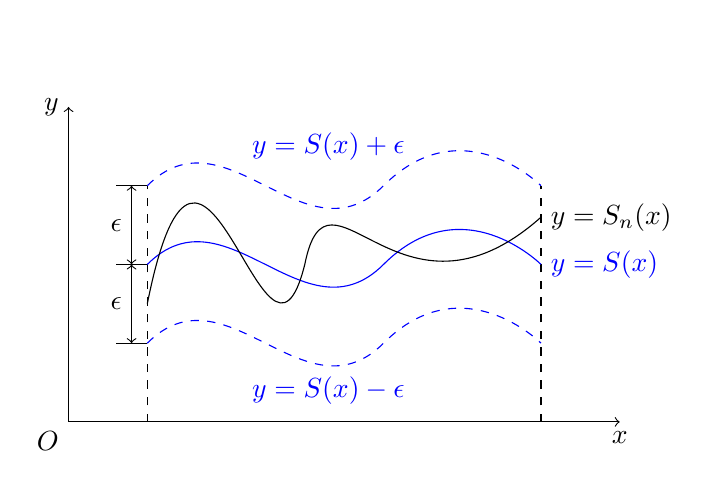
\begin{tikzpicture}
		\draw[->](0,0)node[below left]{\(O\)} -- (7,0)node[below]{\(x\)};
		\draw[->](0,0) -- (0,4)node[left]{\(y\)};
		\draw[dashed](1,0) -- (1,3) (6,0) -- (6,3);
		\draw(1,1)--+(-.4,0);
		\draw(1,2)--+(-.4,0);
		\draw(1,3)--+(-.4,0);
		\begin{scope}[<->,xshift=-.2cm]
			\draw(1,1) -- (1,2)node[midway,left]{\(\epsilon\)};
			\draw(1,2) -- (1,3)node[midway,left]{\(\epsilon\)};
		\end{scope}
		\begin{scope}[blue]
			\draw[dashed] (1,1) .. controls (2,2) and (3,0) .. (4,1) .. controls (5,2) and (6,1) .. (6,1);
			\draw[yshift=1cm] (1,1) .. controls (2,2) and (3,0) .. (4,1) .. controls (5,2) and (6,1) .. (6,1)node[right]{\(y = S(x)\)};
			\draw[yshift=2cm,dashed] (1,1) .. controls (2,2) and (3,0) .. (4,1) .. controls (5,2) and (6,1) .. (6,1);
			\draw(3.3,3.5)node{\(y = S(x) + \epsilon\)};
			\draw(3.3,0.4)node{\(y = S(x) - \epsilon\)};
		\end{scope}
		\draw(1,1.5) .. controls (1.7,5) and (2.5,0) .. (3,2) .. controls (3.3,3.5) and (4.2,1) .. (6,2.6)node[right]{\(y = S_n(x)\)};
	\end{tikzpicture}
	\caption{函数项级数一致收敛的几何解释}
	\label{figure:无穷级数.函数项级数一致收敛的几何解释}
\end{figure}

\begin{proposition}
%@see: 《数学分析(第二版 下册)》(陈纪修) P60 推论10.1.1
若函数项级数\(\sum_{n=1}^\infty u_n\)在\(D\)上一致收敛,
则函数列\(\{u_n\}\)在\(D\)上一致收敛于\(u(x) \equiv 0\).
\begin{proof}
由\cref{definition:无穷级数.函数项级数的一致收敛性} 立即可得.
\end{proof}
\end{proposition}

由于函数项级数的一致收敛性本质上就是部分和函数列的一致收敛性,
所以下面我们仅对函数列举例讨论.

\begin{example}
%@see: 《高等数学(第六版 上册)》 P295 例2
设\(S_n(x) = \frac1{x+n}\).
研究\(\{S_n\}\)在区间\([0,+\infty)\)上的一致收敛性.
\begin{solution}
显然\(S(x) = \lim_{n\to\infty} S_n(x) = 0\).
对于\(\forall\epsilon>0\),
要使\[
	\abs{S(x) - S_n(x)}
	= \frac1{x+n}
	\leq \frac1{n}
	< \epsilon,
\]
可以取\(N \geq \ceil*{\frac1{\epsilon}}\),
当\(n>N\)时,
就有\[
	\abs{S(x) - S_n(x)}
	< \epsilon
\]对一切\(x\in[0,+\infty)\)成立,
因此\(\{S_n\}\)在\([0,+\infty)\)上一致收敛于\(S(x)\equiv0\).
\end{solution}
\end{example}

\begin{example}\label{example:函数项级数.一致收敛的函数列2}
%@see: 《数学分析(第二版 下册)》(陈纪修) P60 例10.1.6
设\(S_n(x) = \frac{x}{1+n^2x^2}\),
则\(\{S_n\}\)在\((-\infty,+\infty)\)上收敛于极限函数\(S(x) = 0\).
这是因为\[
	\abs{S_n(x) - S(x)}
	= \frac{\abs{x}}{1+n^2x^2}
	\leq \frac1{2n},%TODO QUESTION: 怎么放缩成这个只与\(n\)有关的分式的?
\]
所以对任意给定的\(\epsilon>0\),只要取\(N = \floor*{\frac1{2\epsilon}}\),
当\(n>N\)时,就有\[
	\abs{S_n(x) - S(x)} \leq \frac1{2n} < \epsilon
\]对一切\(x\in(-\infty,+\infty)\)成立.

\begin{figure}[htb]
%@see: 《数学分析(第二版 下册)》(陈纪修) P61 图10.1.2
	\centering
	\begin{tikzpicture}
		\begin{axis}[
			name=Plt,
			xscale=1.5,
			xmin=-2.2,xmax=2.2,
			ymin=-.6,ymax=.6,
			axis lines=middle,
			xlabel=$x$,
			ylabel=$y$,
		]
			\addplot[color=red,samples=50,smooth,domain=-2:2]
				{x/(1+x^2)};\label{pgfplots:函数项级数.函数图像1}
			\addplot[color=orange,samples=50,smooth,domain=-2:2]
				{x/(1+4*x^2)};\label{pgfplots:函数项级数.函数图像2}
			\addplot[color=green,samples=50,smooth,domain=-2:2]
				{x/(1+9*x^2)};\label{pgfplots:函数项级数.函数图像3}
			\addplot[color=blue,samples=50,smooth,domain=-2:2]
				{x/(1+25*x^2)};\label{pgfplots:函数项级数.函数图像4}
		\end{axis}
		\node[draw,fill=white,inner sep=0pt,right=1em]
		at(Plt.east){
			\small\begin{tblr}{cl}
				\ref{pgfplots:函数项级数.函数图像1} & \(n=1\) \\
				\ref{pgfplots:函数项级数.函数图像2} & \(n=2\) \\
				\ref{pgfplots:函数项级数.函数图像3} & \(n=3\) \\
				\ref{pgfplots:函数项级数.函数图像4} & \(n=5\) \\
			\end{tblr}
		};
	\end{tikzpicture}
	\caption{}
	\label{figure:函数项级数.图1}
\end{figure}

从几何上看(\cref{figure:函数项级数.图1}),
对任意给定\(\epsilon>0\),只要取\(N = \floor*{\frac1{2\epsilon}}\),
当\(n>N\)时,函数\(S_n\)的图像都落在带状区域\[
	\Set{ (x,y) \given \abs{y} < \epsilon }
\]中,这正是一致收敛的几何描述.
\end{example}

\begin{example}\label{example:函数项级数.不一致收敛的函数列1}
%@see: 《数学分析(第二版 下册)》(陈纪修) P62 例10.1.7
%@see: 《高等数学(第六版 上册)》 P295 例3
设\(S_n(x) = x^n\),
考察\(\{S_n\}\)在区间\([0,1)\)上的一致收敛性.
显然\(S(x) = \lim_{n\to\infty} S_n(x) = 0\).
对任意给定\(\epsilon\in(0,1)\),
要使\[
	\abs{S_n(x) - S(x)} = x^n < \epsilon,
\]
必须\[
	n > \frac{\ln\epsilon}{\ln x},
\]
因此\(N = N(x,\epsilon)\)至少应该取\(\floor*{\frac{\ln\epsilon}{\ln x}}\).
由于当\(x\to1^-\)时,\(\frac{\ln\epsilon}{\ln x}\to+\infty\),
因此不可能找到对一切\(x\in[0,1)\)都适用的\(N = N(\epsilon)\),
换言之,\(\{S_n\}\)在\([0,1)\)上不是一致收敛的.

\begin{figure}[htb]
%@see: 《数学分析(第二版 下册)》(陈纪修) P62 图10.1.3
	\centering
	\begin{tikzpicture}
		\begin{axis}[
			name=Plt,
			xmin=0,xmax=1.2,
			ymin=0,ymax=1.2,
			axis equal=true,
			axis lines=middle,
			xlabel=$x$,
			ylabel=$y$,
		]
			\addplot[color=red,samples=50,smooth,domain=0:1]
				{x};\label{pgfplots:函数项级数.函数图像5}
			\addplot[color=orange,samples=50,smooth,domain=0:1]
				{x^2};\label{pgfplots:函数项级数.函数图像6}
			\addplot[color=green,samples=50,smooth,domain=0:1]
				{x^3};\label{pgfplots:函数项级数.函数图像7}
			\addplot[color=blue,samples=50,smooth,domain=0:1]
				{x^4};\label{pgfplots:函数项级数.函数图像8}
			\draw[dashed,black!30](0,1)--(1,1)--(1,0);
		\end{axis}
		\node[draw,fill=white,inner sep=0pt,right=1em]
		at(Plt.east){
			\small\begin{tblr}{cl}
				\ref{pgfplots:函数项级数.函数图像5} & \(n=1\) \\
				\ref{pgfplots:函数项级数.函数图像6} & \(n=2\) \\
				\ref{pgfplots:函数项级数.函数图像7} & \(n=3\) \\
				\ref{pgfplots:函数项级数.函数图像8} & \(n=4\) \\
			\end{tblr}
		};
	\end{tikzpicture}
	\caption{}
	\label{figure:函数项级数.图2}
\end{figure}

从几何上看(\cref{figure:函数项级数.图2}),
对于每个正整数\(n\),函数\(x \mapsto x^n\)的取值范围(即它的值域)都是\([0,1]\),
因此它们的图像不可能落在带状区域\[
	\Set{ (x,y) \given x\in[0,1), 0<y<\epsilon }
\]中.
\end{example}

\begin{definition}
%@see: 《数学分析(第二版 下册)》(陈纪修) P62 定义10.1.3
若对于任意给定闭区间\([a,b] \subseteq D\),
函数列\(\{S_n\}\)在\([a,b]\)上一致收敛于\(S\),
则称“\(\{S_n\}\)在\(D\)上\DefineConcept{内闭一致收敛}于\(S\)”.
\end{definition}
显然,在\(D\)上一致收敛的函数列必定在\(D\)上内闭一致收敛,
但其逆命题不成立.
例如,将\cref{example:函数项级数.不一致收敛的函数列1} 中
考察的区间\([0,1)\)缩小为\([0,\rho]\),
其中\(0<\rho<1\)是任意的,
则由\[
	\abs{S_n(x) - S(x)} = x^n < \rho^n,
\]
只要取\(N = N(\epsilon) = \floor*{\frac{\ln\epsilon}{\ln\rho}}\),
当\(n>N\)时,就有\[
	\abs{S_n(x) - S(x)} < \rho^n < \epsilon
\]对一切\(x\in[0,\rho]\)成立,
即\(\{S_n\}\)在\([0,\rho]\ (\rho<1)\)上是一致收敛的.
也就是说,尽管\(\{S_n\}\)在\([0,1)\)上不是一致收敛的,
但是它是内闭一致收敛的.

这个例子也说明:函数项级数与函数列的一致收敛性与我们考察的区间有关.

下面我们建立关于一致收敛的两个充分必要条件,它们将有助于对一致收敛性进行判断.
\begin{theorem}\label{theorem:函数项级数.一致收敛的充分必要条件1}
%@see: 《数学分析(第二版 下册)》(陈纪修) P63 定理10.1.1
设函数列\(\{S_n\}\)在集合\(D\)上点态收敛于函数\(S\),
则\(\{S_n\}\)在\(D\)上一致收敛于\(S\)的充分必要条件是:
把\[
	\lim_{n\to\infty} \sup_{x \in D} \abs{S_n(x) - S(x)} = 0.
\]
\begin{proof}
假设\(\{S_n\}\)在集合\(D\)上点态收敛于函数\(S\),
那么对任意给定\(\epsilon>0\),存在正整数\(N = N(\epsilon)\),当\(n>N\)时,有\[
	\abs{S_n(x) - S(x)} < \frac\epsilon2
\]对一切\(x \in D\)成立,
于是\[
	\sup_{x \in D} \abs{S_n(x) - S(x)} \leq \frac\epsilon2 < \epsilon,
\]
这就说明\(\lim_{n\to\infty} \sup_{x \in D} \abs{S_n(x) - S(x)} = 0\).

反过来,假设\(\lim_{n\to\infty} \sup_{x \in D} \abs{S_n(x) - S(x)} = 0\),
则对任意给定\(\epsilon>0\),存在正整数\(N = N(\epsilon)\),当\(n>N\)时,有\[
	\sup_{x \in D} \abs{S_n(x) - S(x)} < \epsilon,
\]
于是\[
	\abs{S_n(x) - S(x)} < \epsilon
\]对一切\(x \in D\)成立,
即\(\{S_n\}\)在\(D\)上一致收敛于\(S\).
\end{proof}
\end{theorem}
回过头来,对于\cref{example:函数项级数.一致收敛的函数列2} 中的
\(S_n(x) = \frac{x}{1+n^2x^2}\ (-\infty < x < +\infty)\),
由于\[
	\abs{S_n(x) - S(x)}
	= \frac{\abs{x}}{1+n^2x^2}
	\leq \frac1{2n}
\]等号成立当且仅当\(x=\pm\frac1n\),
可知\[
	\sup_{-\infty < x < +\infty} \abs{S_n(x) - S(x)}
	= \frac1{2n}
	\to 0
	\quad(n\to\infty),
\]
因此\(\{S_n\}\)在\((-\infty,+\infty)\)上一致收敛于\(S(x)\equiv0\).

对于\cref{example:函数项级数.不一致收敛的函数列1} 中的
\(S_n(x) = x^n\ (0 \leq x < 1)\),
由于\[
	\sup_{0 \leq x < 1} \abs{S_n(x) - S(x)}
	= \sup_{0 \leq x < 1} x^n
	= 1
	\not\to 0
	\quad(n\to\infty),
\]
所以\(\{S_n\}\)在\([0,1)\)上不是一致收敛的.

\begin{example}\label{example:函数项级数.不一致收敛的函数列2}
%@see: 《数学分析(第二版 下册)》(陈纪修) P64 例10.1.8
设\(S_n(x) = \frac{nx}{1+n^2x^2}\),
则\(\{S_n\}\)在\((0,+\infty)\)上收敛于\(S(x)=0\).
由于\[
	\abs{S_n(x) - S(x)}
	= \frac{nx}{1+n^2x^2}
	\leq \frac12
\]等号成立当且仅当\(x=\frac1n\),
可知\[
	\sup_{0 < x < +\infty} \abs{S_n(x) - S(x)}
	= \frac12
	\not\to 0
	\quad(n\to\infty),
\]
因此\(\{S_n\}\)在\((0,+\infty)\)上不是一致收敛的.

\begin{figure}[htb]
%@see: 《数学分析(第二版 下册)》(陈纪修) P64 图10.1.4
	\centering
	\begin{tikzpicture}
		\begin{axis}[
			name=Plt,
			xscale=1.5,
			xmin=0,xmax=4.4,
			ymin=0,ymax=.6,
			axis lines=middle,
			xlabel=$x$,
			ylabel=$y$,
		]
			\addplot[color=red,samples=50,smooth,domain=0:4]
				{x/(1+x^2)};\label{pgfplots:函数项级数.函数图像9}
			\addplot[color=orange,samples=50,smooth,domain=0:4]
				{2*x/(1+4*x^2)};\label{pgfplots:函数项级数.函数图像10}
			\addplot[color=green,samples=50,smooth,domain=0:4]
				{4*x/(1+16*x^2)};\label{pgfplots:函数项级数.函数图像11}
			\addplot[color=blue,samples=50,smooth,domain=0:4]
				{8*x/(1+64*x^2)};\label{pgfplots:函数项级数.函数图像12}
		\end{axis}
		\node[draw,fill=white,inner sep=0pt,right=1em]
		at(Plt.east){
			\small\begin{tblr}{cl}
				\ref{pgfplots:函数项级数.函数图像9} & \(n=1\) \\
				\ref{pgfplots:函数项级数.函数图像10} & \(n=2\) \\
				\ref{pgfplots:函数项级数.函数图像11} & \(n=4\) \\
				\ref{pgfplots:函数项级数.函数图像12} & \(n=8\) \\
			\end{tblr}
		};
	\end{tikzpicture}
	\caption{}
	\label{figure:函数项级数.图3}
\end{figure}

从几何上看(\cref{figure:函数项级数.图3}),
对于每个正整数\(n\),
函数\(x \mapsto \frac{nx}{1+n^2x^2}\)在\(x=\frac1n\)取到最大值\(\frac12\).
因此它们的图像不可能落在带状区域\[
	\Set{ (x,y) \given 0<x<+\infty, \abs{y}<\epsilon<1/2 }
\]中.
事实上,\(\{S_n\}\)在任意包含\(x=0\)或以\(x=0\)为端点的区间上都不是一致收敛的.

若将\(\{S_n\}\)限制在任意有限闭区间\([\rho,A]\ (0<\rho<A<+\infty)\)上,
则由\[
	\abs{S_n(x) - S(x)} = \frac{nx}{1+n^2x^2}
\]及\[
	\dv{x} \left(\frac{nx}{1+n^2x^2}\right)
	= \frac{n(1-n^2x^2)}{(1+n^2x^2)^2},
\]
可以知道当\(n>\frac1\rho\)时,\(\abs{S_n(x) - S(x)}\)在\([\rho,A]\)单调减少,
从而\[
	\sup_{\rho \leq x \leq A} \abs{S_n(x) - S(x)}
	= \frac{n\rho}{1+n^2\rho^2}
	\to 0
	\quad(n\to\infty),
\]
即\(\{S_n\}\)在\([\rho,A]\)上一致收敛于\(S(x)=0\),
或者说\(\{S_n\}\)在\((0,+\infty)\)上内闭一致收敛.
\end{example}

\begin{theorem}\label{theorem:函数项级数.一致收敛的充分必要条件2}
%@see: 《数学分析(第二版 下册)》(陈纪修) P66 定理10.1.2
设函数列\(\{S_n\}\)在集合\(D\)上点态收敛于函数\(S\),
则\(\{S_n\}\)在\(D\)上一致收敛于\(S\)的充分必要条件是:
对任意一个数列\(\{x_n\}\ (x_n \in D)\),
成立\[
	\lim_{n\to\infty} (S_n(x_n) - S(x_n)) = 0.
\]
%TODO proof
\end{theorem}
\cref{theorem:函数项级数.一致收敛的充分必要条件2}
常用于判断函数列的不一致收敛.

\begin{example}
%@credit: {e9b17d8d-3be5-4f44-9c7a-a5e6122a69e2} 提出问题
函数\(f\)在区间\(D\)上一致连续的充分必要条件是:
对于任意一个数列\(\{a_n\}\),
只要\(\lim_{n\to\infty} a_n = 0\),
就有函数列\(\{f(x-a_n)\}\)在\(D\)上一致收敛于\(f\).
\begin{proof}
%@credit: {5a781423-ba4e-4629-ac1a-eac743a4d445} 提供了证明必要性的思路,不用反证法就证明了充分性
%@see: https://math.stackexchange.com/a/4967991/591741 利用反证法,证明充分性
必要性.
假设函数\(f\)在区间\(D\)上一致连续,
则对任意给定\(\epsilon>0\),
存在\(\delta>0\),
对于区间\(D\)上的任意两点\(x_1,x_2\),
当\(\abs{x_1-x_2}<\delta\)时,
有\[
	\abs{f(x_1)-f(x_2)}<\epsilon.
\]
再假设数列\(\{a_n\}\)是任意一个无穷小,
那么对于任意给定\(\delta>0\),
存在正整数\(N\),
当\(n>N\)时,
有\[
	\abs{a_n} < \delta.
\]
于是,对任意给定\(\epsilon>0\),
存在正整数\(N\),
当\(n>N\)时,
对区间\(D\)上的任意一点\(x\),
有\[
	\abs{f(x)-f(x-a_n)}<\epsilon.
\]
这就说明函数列\(\{f(x-a_n)\}\)在\(D\)上一致收敛于\(f\).

充分性.
用反证法.
假设\(f\)在区间\(D\)上不一致连续,
那么存在\(\epsilon_0>0\),
对于任意\(\delta>0\),
存在\(x,y \in D\),
满足\[
	\abs{x-y}<\delta
	\quad\land\quad
	\abs{f(x)-f(y)}\geq\epsilon_0.
\]
于是对于任意正整数\(n\),
存在实数\(x_n,y_n \in D\),
使得\[
	\abs{x_n-y_n}<\frac1n
	\quad\land\quad
	\abs{f(x_n)-f(y_n)}\geq\epsilon_0.
\]
记\(a_n \defeq y_n - x_n\).
显然\(\lim_{n\to\infty} a_n = 0\).
然而,如若假设函数列\(\{f(x-a_n)\}\)在\(D\)上一致收敛于\(f\)成立,
则必定存在正整数\(N\),
当\(n>N\)时,
有\[
	\abs{f(y_n)-f(y_n-a_n)}
	=\abs{f(x_n)-f(y_n)}
	<\epsilon_0,
\]
这与假设矛盾!
这就说明,如果对于任意一个收敛于\(0\)的数列\(\{a_n\}\),
总是成立函数列\(\{f(x-a_n)\}\)在\(D\)上一致收敛于\(f\),
那么函数\(f\)必定在区间\(D\)上一致连续.
\end{proof}
\end{example}
